\section{Implementation}
\label{sec:implementation}
	In this section we discuss the implementation of a generic adaptation
	architecture to realise the
	variation points identified in the previous section. First, we present
	\emph{model adaptation} to address VP1. Afterwards, we discuss how \emph{model
	instance adaptation} supports VP2.
	
	\begin{figure}[p]
			\centering
				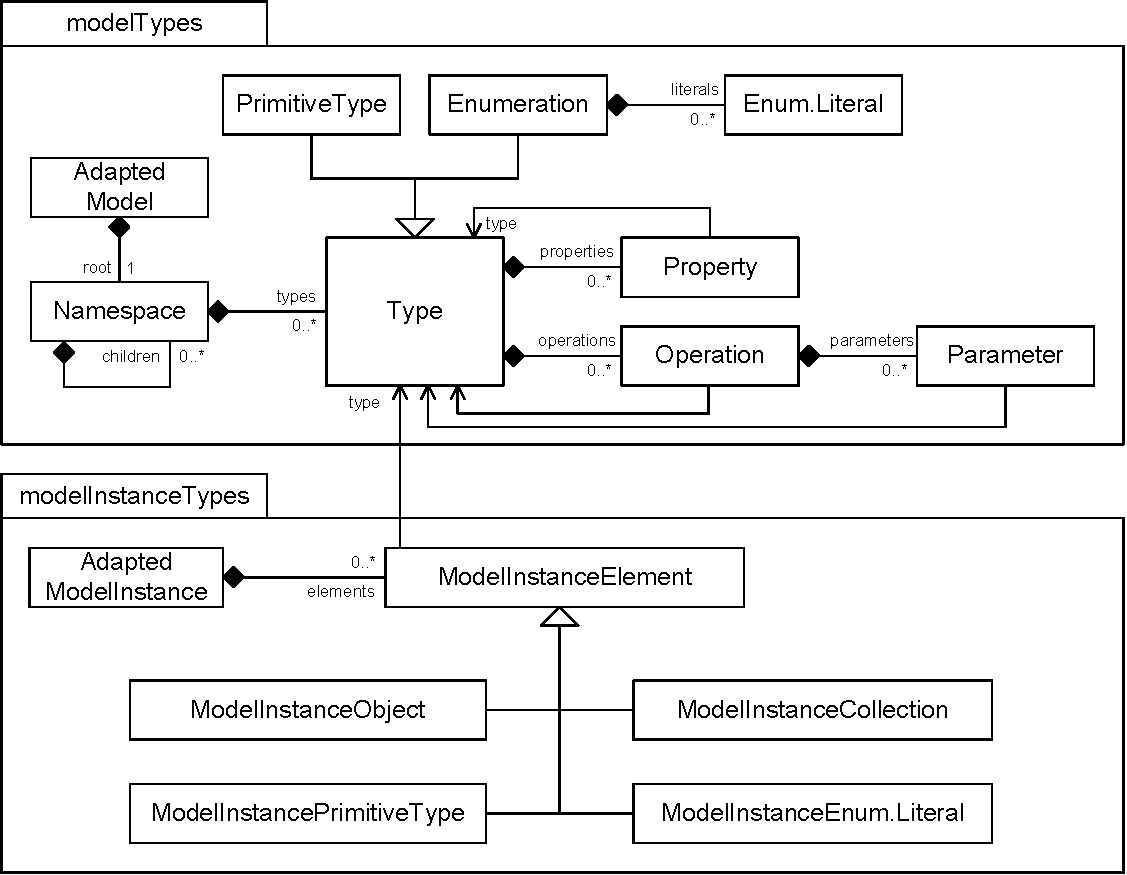
\includegraphics[width=0.80\textwidth]{figures/coreconcepts.pdf}
			\caption{
			Interfaces for model and model instance adaptation
% 			The core concepts of the \emph{Model Types} and \emph{Model Instance Types}:
% 			Each \emph{Model} has a root \emph{Namespace} that contains a set of nested Namespaces and 
% 			a set of \emph{Types}. Each Type has a set of \emph{Operations} 
% 			and \emph{Properties}. 
% 			Each \emph{Model Instance} has a set of \emph{Model Instance Elements}. Each Model Instance
% 			Element has exactly one Type and provides 
% 			operations to reflect on this Type. \emph{Model Instance Objects} provide further reflective 
% 			operations to get properties and to invoke operations.
			}
			\label{fig:coreconcepts}
			
			\vspace{4.0em}
			
				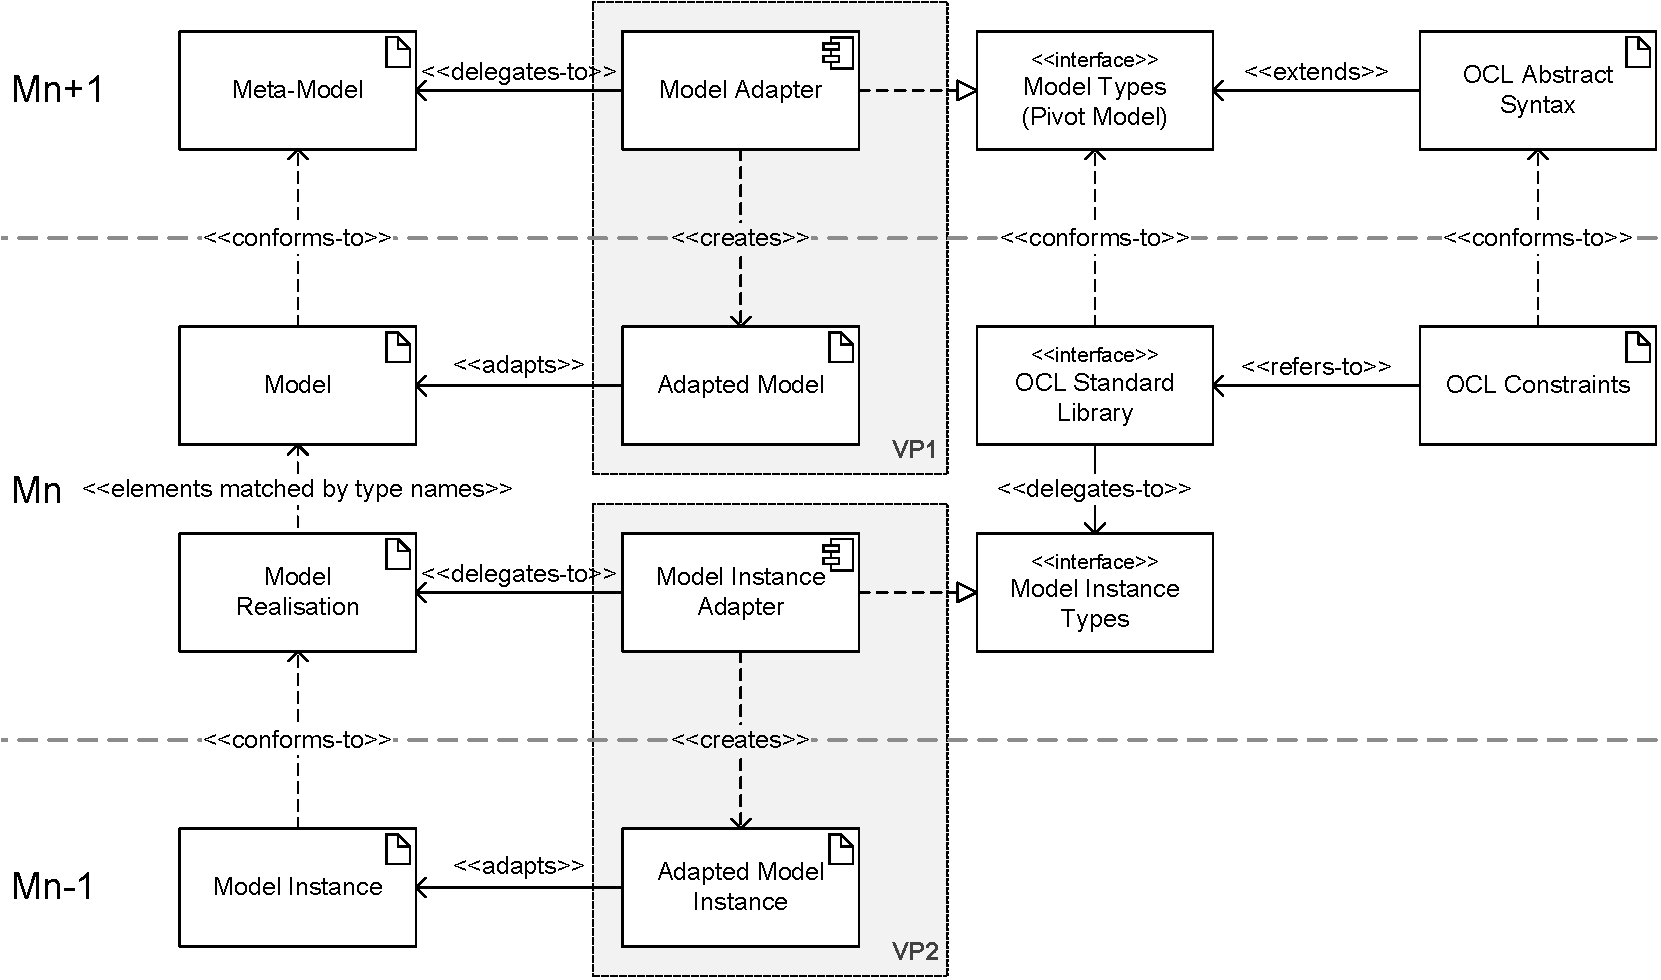
\includegraphics[width=1.00\textwidth]{figures/modeladaptation.pdf}
			\caption{The \emph{Generic Adaptation Architecture} of DresdenOCL
% 			: At the Mn+1 layer, meta-models are adapted
% 			to the Model Types (VP1). The model adapter component contains these adapters and is responsible 
% 			to instantiate them to adapt models of the meta-model. 
% 			At the Mn layer, model implementation types are adapted (VP2). The model instance adapter component
% 			contains these adapters and is responsible to instantiate them to adapt model instance objects. 
% 			The OCL standard library implements the logic to evaluate operations defined on OCL types. Other 
% 			requests such as operation invocations or property requests on adapted objects are delegated 
% 			via the interfaces of the model implementation type model.
			}
			\label{fig:modeladaptation}			
		\end{figure}

\subsection{Model Adaptation (VP1)}

	In order to define OCL constraints for various models,
	DresdenOCL provides a set of common interfaces abstracting structures
	that are required to navigate and query models.
	These interfaces~--~called \texttt{modelTypes} (or \texttt{pivotModel})~\cite{braeuerOCL07}~--~define
	the basic	concepts such as \texttt{Type}, \texttt{Property}, \texttt{Operation} and \texttt{Parameter}
	that bind OCL constraints to a concrete model (cf. Fig. \ref{fig:coreconcepts}).
	DresdenOCL uses these concepts to parse and statically analyse OCL constraints, 
	e.g., the OCL parser can determine the \texttt{Type} of OCL expressions.
	
	For every model that shall be connected with DresdenOCL, 
	a \emph{model adapter} component has to be implemented (cf. Fig. \ref{fig:modeladaptation}, Mn+1 layer). 
	It contains individual adapters that map concepts of the model to corresponding artefacts of the \texttt{modelTypes}. E.g., the UML
	meta-model concept \texttt{UMLClass} is adapted to the \texttt{modelTypes} concept
	\texttt{Type}. 
	Furthermore, the model adapter component has to create 
	adapters on demand resulting in an \textit{adapted model} (cf. Fig.
	\ref{fig:modeladaptation}, Mn layer).
	The adapters are only created for model elements that are required and
	existing adapters are cached. Thus, unnecessary and expensive adaptation is avoided, 
	especially when working on large models of which only parts are constrained.
% 	The presented architecture provides a generic and easy variation of multiple meta-models
% 	and corresponding models in an OCL infrastructure (VP1).


\subsection{Model Instance Adaptation (VP2)}
	
% 	The presented abstraction of Model Types to support various models
% 	and meta-models can now be shifted and extended to
% 	solve similar problems when working with multiple model instantiations. 
	In our generic adaptation architecture we applied the same principles for model instances as those are also hidden behind a set of common
	interfaces. This enables the reuse of the same OCL interpreter for the dynamic
	evaluation of OCL constraints on model instances with various realisation techniques.
	
	To provide means for model instance adaptation, we introduced the
	\texttt{model\-Instance\-Types}. The \texttt{modelInstanceTypes} are a set of \texttt{ModelInstanceElements}
	representing instances of primitive types, 
	collections and objects defined in the model (cf. Fig. \ref{fig:coreconcepts}). 
  The most important difference between the \texttt{modelTypes} and \texttt{modelInstanceTypes}
	is that \texttt{modelTypes} abstract modelling concepts whereas \texttt{modelInstanceTypes} abstract 
	reflection capabilities of different model instances (cf. Fig. \ref{fig:modeladaptation}, Mn and Mn-1 layer).
	During interpretation, the OCL interpreter uses the reflection mechanism to
	retrieve the \texttt{Type} of a \texttt{ModelInstanceElement}, to access \texttt{Property}
	values, or to invoke \texttt{Operations}.
	
	Each kind of model instance that shall be connected with DresdenOCL is
	adapted via a \emph{model instance adapter} component (cf. Fig.
	\ref{fig:modeladaptation}, Mn layer). The model instance adapter component contains adapters that map elements of a
	concrete model instance to \texttt{modelInstanceTypes} and has to
	create \texttt{Model\-Instance\-Elements} for the runtime 
	objects of the adapted model instance (cf. Fig. \ref{fig:modeladaptation}, Mn-1 layer). 
	The model instance adapter component also 
	creates adapters for objects on demand. Adapted objects are cached to
	improve the performance and to avoid phenomena like \emph{object
	schizophrenia} \cite{assmann:isc}.\note{Claas: Reference Okay? Christian:
	Didn't florian send the original source? Always use the most concrete you know. Claas: The other references talk
	about Split Objects (reason) and not about the phenomenon. We have to discuss this on Monday.}
	
	% said a few times before 
	%
	%Due to the introduction of a common set of Model Instance Types it is possible
	%to easily reuse the same OCL interpreter for various kinds of model
	%instances. Thus, VP2 can be completely addressed by the presented generic
	%adapter architecture.


